\documentclass{sig-alternate-10pt}

\usepackage{graphics}
\usepackage{epsfig}
%\usepackage{appendix}
\usepackage{color}
\usepackage[usenames,dvipsnames]{xcolor}
\usepackage{url}
\usepackage{underscore}

\usepackage{times}

%
% Get rid of excess white space, commands copied from:
% http://www.terminally-incoherent.com/blog/2007/09/19/latex-squeezing-the-vertical-white-space/
%
\usepackage{mdwlist}

%SOME USEFUL COMMANDS
% Use: \paragraphb{Blah}: blah blah -- this will make the paragraph start with bold text and not be indented
%    : (\eg Blah) -- will add the text e.g., in italics
%    : \comment{Blah} -- will add the text in braces in a certain color

\newcommand{\eg}{{\em e.g., }}
\newcommand{\ie}{{\em i.e., }}
\newcommand{\paragraphb}[1]{\vspace{0.03in}\noindent{\bf #1} }
\newcommand{\paragraphe}[1]{\vspace{0.03in}\noindent{\em #1} }
\newcommand{\paragraphbe}[1]{\vspace{0.03in}\noindent{\bf \em #1} }
\newcommand{\comment}[1]{\textcolor{purple}{#1}}

\title{Spiffy Title Here}

\author{Kelly Nicole Kaoudis, Alexander Campbell, Eric Keller \\
\{kaoudis, alexander.campbell, eric.keller\}@colorado.edu}

\begin{document}
\setlength{\pdfpagewidth}{8.5in}
\setlength{\pdfpageheight}{11in}

\thispagestyle{empty}

\maketitle


%% Have one file per section, and include them all here

\begin{abstract}
You put an abstract here.
\end{abstract}

\section{Introduction}
\label{sec:intro}

In researching and constructing this system, we had three main
objectives in mind.

\subsubsection*{Security}

While the Internet is a multinational, borderless entity, its
cultural heritage is based in the expectation that \textit{all}
users may speak freely and exchange information and ideas with
anyone, at any time. Tor, Freenet, and I2P all claim to
allow their users to transfer and/or receive information without
exposure of real-world credentials such as legal names and
IP addresses. These services are utilized across demographics
and national boundaries. This speaks to a strong desire for
uncensored communication and information sharing.

The United Nations' Universal Declaration of Human Rights details
certain freedoms to which all individuals are entitled. Its
twelfth and nineteenth articles in particular, similarly to the
First Amendment to the United States Constitution and Section 2b
of the Canadian Charter of Rights and Freedoms, paraphrased,
state that all humans should have the
right to freedom of expression and
opinion and should not be subject to arbitrary interference with
their assembly and privacy.

In the interest of a more open Internet where information may be
shared freely regardless of national and political differences,
security and user privacy must be primary considerations for
developers whose applications deal with users' personal data.
When security is not a bolt-on afterthought but is initially
important, one's work becomes more difficult to compromise.

\subsubsection*{Usability}

We are also concerned with the ability of our users to easily
understand and employ our service without accidentally revealing
personally identifiable information or other data they do not
want shared. Our system should offer the fewest (unpleasant)
surprises possible to the user both in terms of how the interface
works and that their data is actually secure.

While Tor and similar services were designed with some measure
of usability in mind, we argue that it is quite possible to do
better, particularly in light of recent breaches of cloud
filesharing services as well as crackdowns on Tor hidden service
operators.

The general public has been trained to expect the convenience of
being able to launch any sort of application with little fuss.
Popular virtual private storage / storage as a
service providers do little to contradict (or even prove correct
by implementing and continuously improving more secure systems)
the belief that properly securing data is trivial,
or that one's data will be secure at
all once entrusted to the service provider.

With Tor particularly, it is easy to misconfigure some aspect
of one's personal browsing or hidden service setup without
at least some knowledge of the inner workings of Internet
security and privacy technologies.

Further, Snowden argues that some possible adversaries are
capable of a trillion hashes per second. It therefore is logical
to make our system as simple, transparent, and \textit{ironclad}
as we possibly can. We use as much layered, strong encryption as
we can manage without overcomplicating the user experience (or the
back end code) as well as a few lessons learned from the best
points of Tor, I2p, and Freenet to do our best to deliver to
users' expectations that the integrity of their data has not
been undermined.

\subsubsection*{Simplicity}

Each component should do just one thing. It should be simple
for future developers to explore and test new as well as existing
functionality, or even extend this work in new directions.
Each of our components should be designed and tested with limited
reliance on elements belonging to other components.
The simpler and more sturdy a system and its parts are, the easier
it is to reuse parts or extend them (and the more likely we
are to convince others to hack on and improve our ideas).

During the beginning of the implementation process, we realized
our design at the time used a lot of moving parts simply because
the technology was interesting, new, or partially solved a problem.
Byzantine faults are more likely in a more complicated system.
\textit{Failure} due to Byzantine faults is both common to many
sorts of distributed systems and potentially exploitable by
attackers. The less complicated and more streamline our system
becomes, the more easy it will be to implement redundancy and
guard against `benign' as well as malicious faults and failures.

%Probably also say something about DHT's here

\section{Related Work}

We present relevant apects of selected work in the anonymity and
distributed filesharing domains from which we have taken inspiration.

\subsubsection*{Why Johnny can't stay anonymous}

Johnny can't encrypt if the secure applications available to him are non-intuitive and difficult for
less technical users to properly employ. Whitten et al discovered by way of lab trials that PGP's
user interface was difficult to use and understand even for people with some technical background,
at time of publication.

While the field of user experience has since made huge progress and is one of the foremost design
concerns in application architecture, usability is still less frequently considered when applications,
tools, and frameworks for security and privacy are developed. If Johnny has information he needs
to get to Alice without those with a lot of computing power at their disposal virtually reading over
his shoulder, he should not need to become an expert in low-level topics in order to properly configure
and utilize such services as will let him encrypt, sign, send, and receive data with zero interference
by any third parties (including the service provider) and little fuss.

Suppose Johnny is a journalist, activist, or really anyone with low technical expertise who might be working
somewhere with business practices on the shady side that are actively hurting people.
If services such as anonymous filesharing are difficult to understand and use, Johnny might not be able to get the
word out. He might even be detained or arrested if visible use of such services is against local law. We
propose creating a simple client-facing application and making its source available for public, version-controlled
contribution in order to ensure such a service remains freely available.

\subsubsection*{Tor and the onion protocol}

Tor is a widely used, well-documented project claiming to provide more security than its users would have openly
conducting business. The Tor FAQ states that peer-to-peer filesharing is not desired (or to be a focus of operation)
within the Tor network. Data such as IP addresses sent over UDP-based P2P protocols are not anonymized by Tor or
SOCKS proxies in general.

Further, due (we hypothesize) to Tor's notoriety in mainstream media and additionally the general public's lack of
understanding of Tor's inner workings, the number of people who contribute back by running nodes
or improving the codebase is much smaller than the number of people merely using the service to protect themselves.
We find this situation analogous to most P2P networks' leechers-versus-seeders situation, in which those who download
and then do not actively seed typically outnumber those that download and then seed files to others.
The number of those who run exit nodes (a crucial part of the Tor infrastructure) is smallest of all, due to a history of
abuse by malicious users and backlash from ISPs. Systems such as TorWard are being developed to assess and reduce the
risk of ill-meaning traffic to exit node operators and other Tor volunteers, but work in this space is relatively nascent.

Tor uses an incremental path-building design: each successive hop in a \textit{circuit}, which is a path between a user's entry
point and her destination, negotiates its own session keys to provide each acting node in a circuit a sort of plausible
deniability. In our own design, transport of a given chunk of data from
the user to the DHT node which her client has chosen as that chunk's eventual destination is modelled closely
after these circuits.

In addition to letting users browse relatively securely,
Tor offers its users the ability to set up \textit{hidden services}, or alternatives to sites on the open web offering anything
servable over a SOCKS proxy. While the idea is that operating such a service would be anonymous in that the operator's
IP address, name, physical location, and other personal details should not be revealed, it has been shown that this isn't
the most reliable or safe practice. Hidden services, by way of a \textit{hidden service descriptor},
which consists of the service's public key and a list of its
acknowledged introduction points (relays that act essentially like human translators in relaying traffic between site
accessors and the site itself) can advertise themselves in a globally available directory.

Furthermore it has been shown using the Cisco traffic analysis tool Netflow that it is possible to uncloak around 81\% of
Tor users, particularly in cases where the users did not properly configure their setups. While we strongly advocate for
an improved Tor, we believe our system combines its better points with the ease of peer-to-peer transactions.

\subsubsection*{I2p}

Somewhat like Tor in purpose, I2p is an anonymous network based around the \textit{I2p router}. I2p is designed to work
atop the bespoke UDP and TCP-like protocols SSU and NTCP. These protocols run atop the peer-to-peer network, which itself
sits on top of IP. All peer and service metadata is stored in a distributed hash table called
\textit{netDB}. Network database records are stored in a Kademlia-like DHT \textit{floodfill}.
Since netDB is run alongside regular I2p nodes, it may be considered less a trusted
group of authorities than functionally interwoven in the network.

All connections inside I2p's inclusive \textit{darknet} are end-to-end encrypted; the router multiplexes theses connections over
pairs of single-direction \textit{I2p tunnels}, which are (when considered as a pair) analogous to Tor's circuits. These tunnels
are constructed with the onion protocol. All participants are meant to remain anonymous, though in practice this does not always
appear to be the case. I2p is a much smaller project than Tor; this means fewer users providing white noise to mask one's traffic,
fewer developers, and fewer volunteers running nodes and services.

Additionally, at time of writing the port of the secure distributed Tahoe filesystem allowing decentralized storage similar
to Freenet on top of I2p is not maintained, and is not up to date with the current version of the filesystem. The largest difference
between Tahoe and Freenet, according to Tahoe's creators, is that file distribution in Freenet is totally random and that secure
usage of Tahoe depends on having a large network of friends and family one can shoehorn into also using the system, since Tahoe assumes
discovery of storage happens out-of-band. Further, Tahoe makes no attempt to obscure the source or destination of
requests. While it is exceedingly difficult to guarantee a
high probability of remaining anonymous against sophisticated attackers, that doesn't mean trying to (and explicitly stating that
use of the service is at one's own risk) isn't worthwhile.

\subsubsection*{Freenet}

Freenet is a location-independent peer-to-peer distributed filesystem of nodes that collaborate to store and retrieve encrypted files,
which are named by 160-bit SHA1 hashes that do not depend on the files' locations. Each user maintains their own \textit{local} datastore
contribution that stores a randomized assortment of other users' data as a portion of their hard drive (which might otherwise go
under-utilized). Freenet maintains a \textit{hops-to-live} value analogoous to
the ICMP time-to-live on active requests for files, which is decremented at each node the request reaches, to prevent infinite cycling
through the system.

We improve on the somewhat risky-seeming practice of safeguarding others' data on one's own machine by moving our
users' data storage contributions offsite to virtual private storage instances.
Additionally we repurpose the \textit{hops-to-live} idea to additionally limit the number of
downloads that may take place before the space in our distributed filesystem dedicated to a file's chunks and identifier will be
repurposed to hold other information (Freenet uses an LRU caching policy to determine whhat gets deleted when from an individual node
when there is not enough space).

\subsubsection*{CYRUS} % talk more about sangtae's paper

CYRUS is a secure data-sharing system to be used amongst one's own devices. One of the things most interesting about CYRUS is it relies
upon the concept of \textit{secret sharing}: that is, a piece of data is broken into chunks and can be reconstructed from any of those
chunks. We believe this is both highly useful for fault tolerance and incredibly insecure; for now we have chosen to improve on this
method by encrypting our data before it is chunked and sent into our distributed hash table, but future refining of this idea is highly
possible.

Another notable feature of CYRUS is its simple, intiuitive, and clean user interface.
Currently it can only be used on iOS, which we believe is a bit
of a drawback, but porting to other operating systems and so on is a relatively easy task. We chose (instead of creating a native
application) to write our clientside interface entirely in Javascript, specifically node.js, so that it can simply be opened locally
in any browser. While others may disagree with our choice to not host this application ourselves, we believe it is more secure for users
to simply start the application, point their browser at localhost, and therefore have their data encrypted and chunked before
it leaves their local machine.

\subsubsection*{BitTorrent} % and kademlia tables

BitTorrent's internal distributed hash table extension, which is based on the Kademlia model and allows for the tracking of peers without
a standard tracker, initially inspired much of this work, though the BitTorrent routing protocol (and the DHT extension) are far more
complicated than would suit our needs. Further, trackerless torrent groups often require the disclosure of some identifying
information to join, are not widely publicised, and are typically used for distribution of material copyrighted by others.

We do not want to employ the idea of ``peers" except between nodes in our DHT: our hash table
is essentially a multiway peer-to-peer network, tracked by a globally (publicly) available ``peer list" that is updated by each new
node when it joins the content store. We utilize the idea of ``trackerless torrents" as well to leave less of a paper trail for data
transfers between nodes, which are designed to firstly ensure no single node knows exactly what it is storing and secondly to keep
the sum total of the content in the data store balanced across all currently available nodes.

% talk about Kademlia and how it works

% talk more about how BT uses it?

\subsubsection*{Bamboo} %super sweet dht which we are going to use

Bamboo (OpenDHT's distributed hash table) relies on a routing algorithm called Chord-FRT. While we originally planned to implement our
own distributed hash table and routing algorithm, Chord-FRT did nearly everything we planned to include in our version. Commands include
GET, PUT, and RM: GET requests a chunk of data to the table, PUT adds data, and an RM request will (eventually) remove a file once the
node to which the RM was issued comes in contact with a piece of that file.

We chose to organize our chunks of information in each node of the DHT via a key,value data store. We improve upon the security of adding
items to and removing items from Bamboo by implementing onion routing from the client to an item's eventual resting place: each ``hop",
from the client to the edge node it has made initial contact with, and from that edge node through the DHT, negotiates its own session keys
and removes a layer of the ``onion" from the data chunk as the chunk is passed through. We will speak more in detail to this later.


\section{Related Work}

We present relevant apects of selected work in the anonymity and
distributed filesharing domains from which we have taken inspiration.

\subsubsection*{Why Johnny can't stay anonymous}

Johnny can't encrypt if the secure applications available to him are non-intuitive and difficult for
less technical users to properly employ. Whitten et al discovered by way of lab trials that PGP's
user interface was difficult to use and understand even for people with some technical background,
at time of publication.

While the field of user experience has since made huge progress and is one of the foremost design
concerns in application architecture, usability is still less frequently considered when applications,
tools, and frameworks for security and privacy are developed. If Johnny has information he needs
to get to Alice without those with a lot of computing power at their disposal virtually reading over
his shoulder, he should not need to become an expert in low-level topics in order to properly configure
and utilize such services as will let him encrypt, sign, send, and receive data with zero interference
by any third parties (including the service provider) and little fuss.

Suppose Johnny is a journalist, activist, or really anyone with low technical expertise who might be working
somewhere with business practices on the shady side that are actively hurting people.
If services such as anonymous filesharing are difficult to understand and use, Johnny might not be able to get the
word out. He might even be detained or arrested if visible use of such services is against local law. We
propose creating a simple client-facing application and making its source available for public, version-controlled
contribution in order to ensure such a service remains freely available.

\subsubsection*{Tor and the onion protocol}

Tor is a widely used, well-documented project claiming to provide more security than its users would have openly
conducting business. The Tor FAQ states that peer-to-peer filesharing is not desired (or to be a focus of operation)
within the Tor network. Data such as IP addresses sent over UDP-based P2P protocols are not anonymized by Tor or
SOCKS proxies in general.

Further, due (we hypothesize) to Tor's notoriety in mainstream media and additionally the general public's lack of
understanding of Tor's inner workings, the number of people who contribute back by running nodes
or improving the codebase is much smaller than the number of people merely using the service to protect themselves.
We find this situation analogous to most P2P networks' leechers-versus-seeders situation, in which those who download
and then do not actively seed typically outnumber those that download and then seed files to others.
The number of those who run exit nodes (a crucial part of the Tor infrastructure) is smallest of all, due to a history of
abuse by malicious users and backlash from ISPs. Systems such as TorWard are being developed to assess and reduce the
risk of ill-meaning traffic to exit node operators and other Tor volunteers, but work in this space is relatively nascent.

Tor uses an incremental path-building design: each successive hop in a \textit{circuit}, which is a path between a user's entry
point and her destination, negotiates its own session keys to provide each acting node in a circuit a sort of plausible
deniability. In our own design, transport of a given chunk of data from
the user to the DHT node which her client has chosen as that chunk's eventual destination is modelled closely
after these circuits.

In addition to letting users browse relatively securely,
Tor offers its users the ability to set up \textit{hidden services}, or alternatives to sites on the open web offering anything
servable over a SOCKS proxy. While the idea is that operating such a service would be anonymous in that the operator's
IP address, name, physical location, and other personal details should not be revealed, it has been shown that this isn't
the most reliable or safe practice. Hidden services, by way of a \textit{hidden service descriptor},
which consists of the service's public key and a list of its
acknowledged introduction points (relays that act essentially like human translators in relaying traffic between site
accessors and the site itself) can advertise themselves in a globally available directory.

Furthermore it has been shown using the Cisco traffic analysis tool Netflow that it is possible to uncloak around 81\% of
Tor users, particularly in cases where the users did not properly configure their setups. While we strongly advocate for
an improved Tor, we believe our system combines its better points with the ease of peer-to-peer transactions.

\subsubsection*{I2p}

Somewhat like Tor in purpose, I2p is an anonymous network based around the \textit{I2p router}. I2p is designed to work
atop the bespoke UDP and TCP-like protocols SSU and NTCP. These protocols run atop the peer-to-peer network, which itself
sits on top of IP. All peer and service metadata is stored in a distributed hash table called
\textit{netDB}. Network database records are stored in a Kademlia-like DHT \textit{floodfill}.
Since netDB is run alongside regular I2p nodes, it may be considered less a trusted
group of authorities than functionally interwoven in the network.

All connections inside I2p's inclusive \textit{darknet} are end-to-end encrypted; the router multiplexes theses connections over
pairs of single-direction \textit{I2p tunnels}, which are (when considered as a pair) analogous to Tor's circuits. These tunnels
are constructed with the onion protocol. All participants are meant to remain anonymous, though in practice this does not always
appear to be the case. I2p is a much smaller project than Tor; this means fewer users providing white noise to mask one's traffic,
fewer developers, and fewer volunteers running nodes and services.

Additionally, at time of writing the port of the secure distributed Tahoe filesystem allowing decentralized storage similar
to Freenet on top of I2p is not maintained, and is not up to date with the current version of the filesystem. The largest difference
between Tahoe and Freenet, according to Tahoe's creators, is that file distribution in Freenet is totally random and that secure
usage of Tahoe depends on having a large network of friends and family one can shoehorn into also using the system, since Tahoe assumes
discovery of storage happens out-of-band. Further, Tahoe makes no attempt to obscure the source or destination of
requests. While it is exceedingly difficult to guarantee a
high probability of remaining anonymous against sophisticated attackers, that doesn't mean trying to (and explicitly stating that
use of the service is at one's own risk) isn't worthwhile.

\subsubsection*{Freenet}

Freenet is a location-independent peer-to-peer distributed filesystem of nodes that collaborate to store and retrieve encrypted files,
which are named by 160-bit SHA1 hashes that do not depend on the files' locations. Each user maintains their own \textit{local} datastore
contribution that stores a randomized assortment of other users' data as a portion of their hard drive (which might otherwise go
under-utilized). Freenet maintains a \textit{hops-to-live} value analogoous to
the ICMP time-to-live on active requests for files, which is decremented at each node the request reaches, to prevent infinite cycling
through the system.

We improve on the somewhat risky-seeming practice of safeguarding others' data on one's own machine by moving our
users' data storage contributions offsite to virtual private storage instances.
Additionally we repurpose the \textit{hops-to-live} idea to additionally limit the number of
downloads that may take place before the space in our distributed filesystem dedicated to a file's chunks and identifier will be
repurposed to hold other information (Freenet uses an LRU caching policy to determine whhat gets deleted when from an individual node
when there is not enough space).

\subsubsection*{CYRUS} % talk more about sangtae's paper

CYRUS is a secure data-sharing system to be used amongst one's own devices. One of the things most interesting about CYRUS is it relies
upon the concept of \textit{secret sharing}: that is, a piece of data is broken into chunks and can be reconstructed from any of those
chunks. We believe this is both highly useful for fault tolerance and incredibly insecure; for now we have chosen to improve on this
method by encrypting our data before it is chunked and sent into our distributed hash table, but future refining of this idea is highly
possible.

Another notable feature of CYRUS is its simple, intiuitive, and clean user interface.
Currently it can only be used on iOS, which we believe is a bit
of a drawback, but porting to other operating systems and so on is a relatively easy task. We chose (instead of creating a native
application) to write our clientside interface entirely in Javascript, specifically node.js, so that it can simply be opened locally
in any browser. While others may disagree with our choice to not host this application ourselves, we believe it is more secure for users
to simply start the application, point their browser at localhost, and therefore have their data encrypted and chunked before
it leaves their local machine.

\subsubsection*{BitTorrent} % and kademlia tables

BitTorrent's internal distributed hash table extension, which is based on the Kademlia model and allows for the tracking of peers without
a standard tracker, initially inspired much of this work, though the BitTorrent routing protocol (and the DHT extension) are far more
complicated than would suit our needs. Further, trackerless torrent groups often require the disclosure of some identifying
information to join, are not widely publicised, and are typically used for distribution of material copyrighted by others.

We do not want to employ the idea of ``peers" except between nodes in our DHT: our hash table
is essentially a multiway peer-to-peer network, tracked by a globally (publicly) available ``peer list" that is updated by each new
node when it joins the content store. We utilize the idea of ``trackerless torrents" as well to leave less of a paper trail for data
transfers between nodes, which are designed to firstly ensure no single node knows exactly what it is storing and secondly to keep
the sum total of the content in the data store balanced across all currently available nodes.

% talk about Kademlia and how it works

% talk more about how BT uses it?

\subsubsection*{Bamboo} %super sweet dht which we are going to use

Bamboo (OpenDHT's distributed hash table) relies on a routing algorithm called Chord-FRT. While we originally planned to implement our
own distributed hash table and routing algorithm, Chord-FRT did nearly everything we planned to include in our version. Commands include
GET, PUT, and RM: GET requests a chunk of data to the table, PUT adds data, and an RM request will (eventually) remove a file once the
node to which the RM was issued comes in contact with a piece of that file.

We chose to organize our chunks of information in each node of the DHT via a key,value data store. We improve upon the security of adding
items to and removing items from Bamboo by implementing onion routing from the client to an item's eventual resting place: each ``hop",
from the client to the edge node it has made initial contact with, and from that edge node through the DHT, negotiates its own session keys
and removes a layer of the ``onion" from the data chunk as the chunk is passed through. We will speak more in detail to this later.


\section{System Architecture}
\label{sec:arch}

Here are some epic diagrams of wtf we built.

\begin{center}
    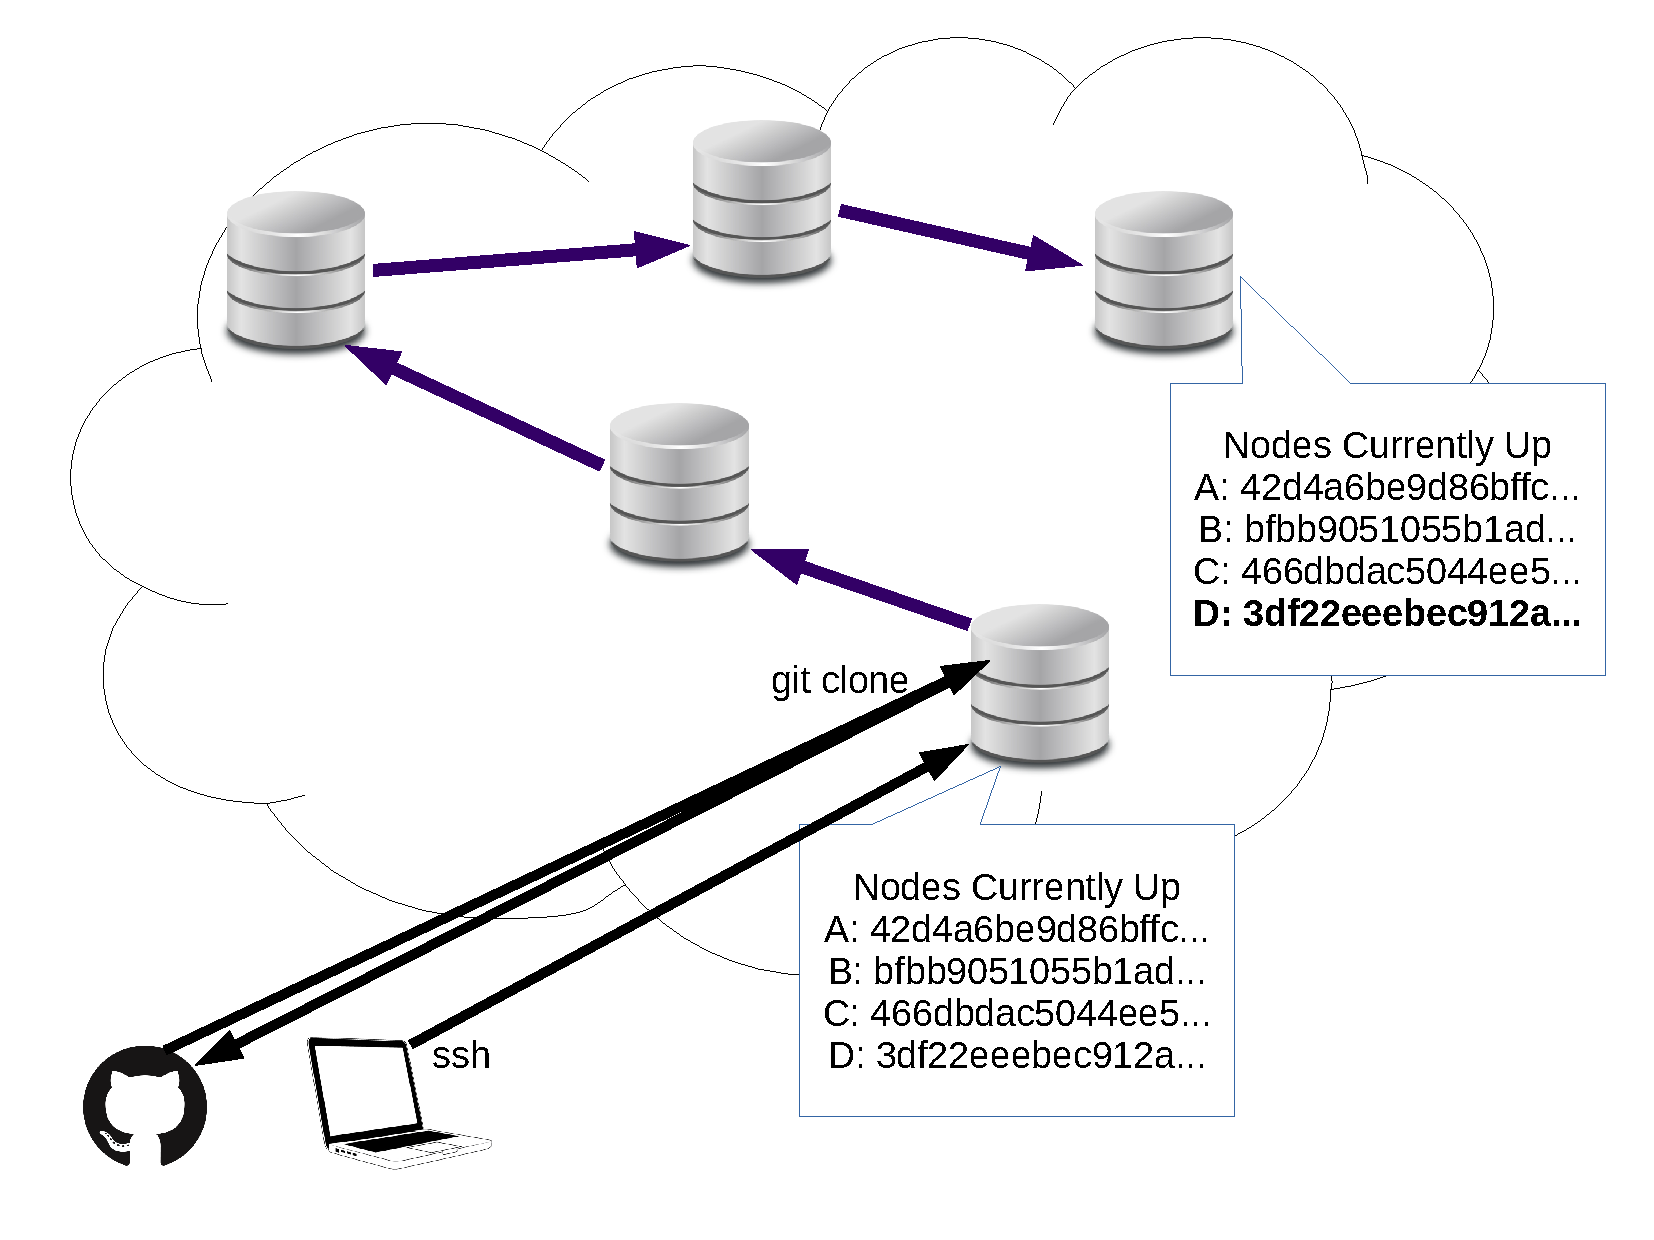
\includegraphics[scale=0.3]{figs/addingaNode.pdf}
    \\
    \small{Adding a node to the network consists of several steps. First, one needs to either obtain a VPS instance or
    server space elsewhere. Secondly, one must ssh in and `git clone' our node repo, then run an install script and
    ensure firewall settings allow inbound and outbound TCP connections from all nodes on the Up List. As load balancing
    occurs, the full amount of storage offered through the new node will be utilized -- it may take a few days.}
    \\
\end{center}

Again let's reiterate how we are different from the projects in our related works section

Describe user experience stuff

\begin{center}
    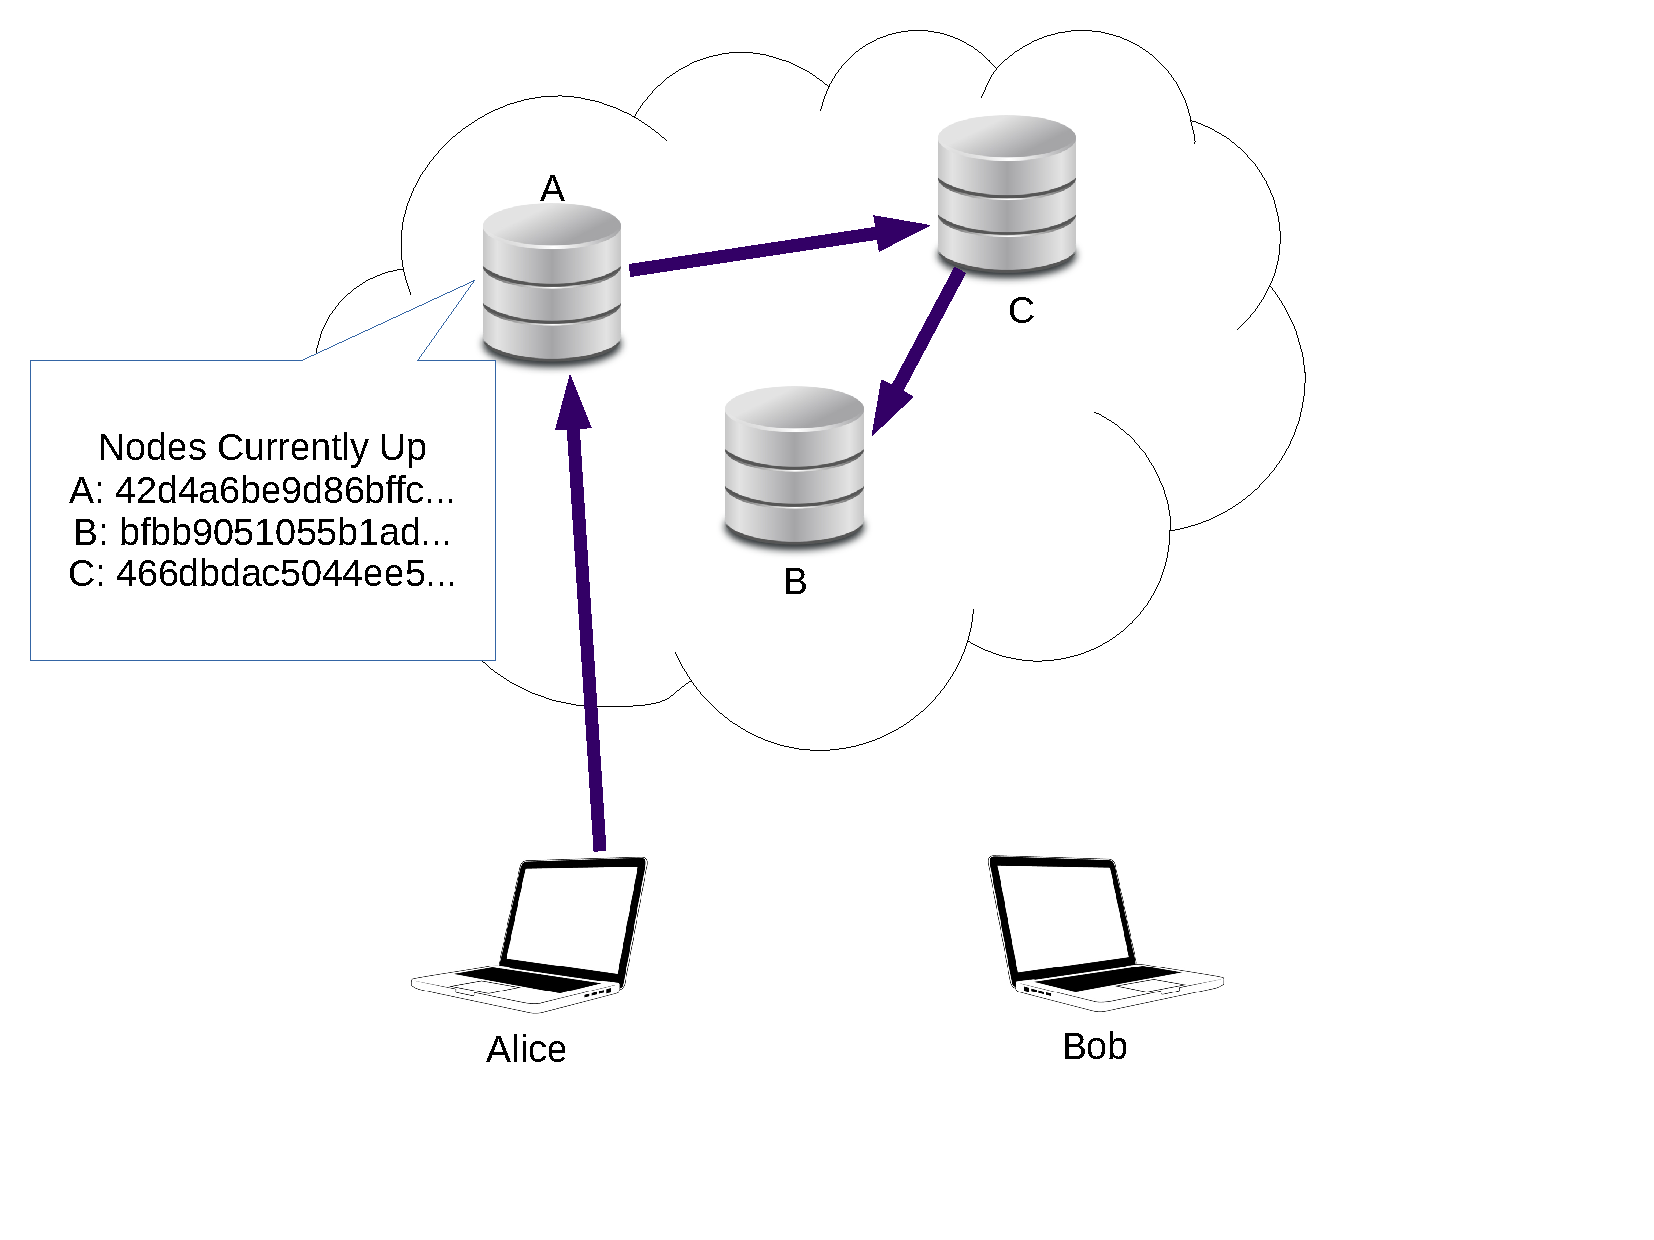
\includegraphics[scale=0.35]{figs/upload.pdf}
    \\
    \small{Uploading to the service is as simple as drag-and-drop. Within Alice's client application, the ``dropped" file
    is encrypted, and the encrypted version of the file is hashed. The encrypted file is then broken up into chunks and
    transported via PUT requests to multiple entry point nodes in the data store via several circuits.
    Each circuit constructed from Alice to
    the data store should have multiple data chunks from different parts of the file or set of files sent over it in random
    order.}
    \\
\end{center}

\begin{center}
    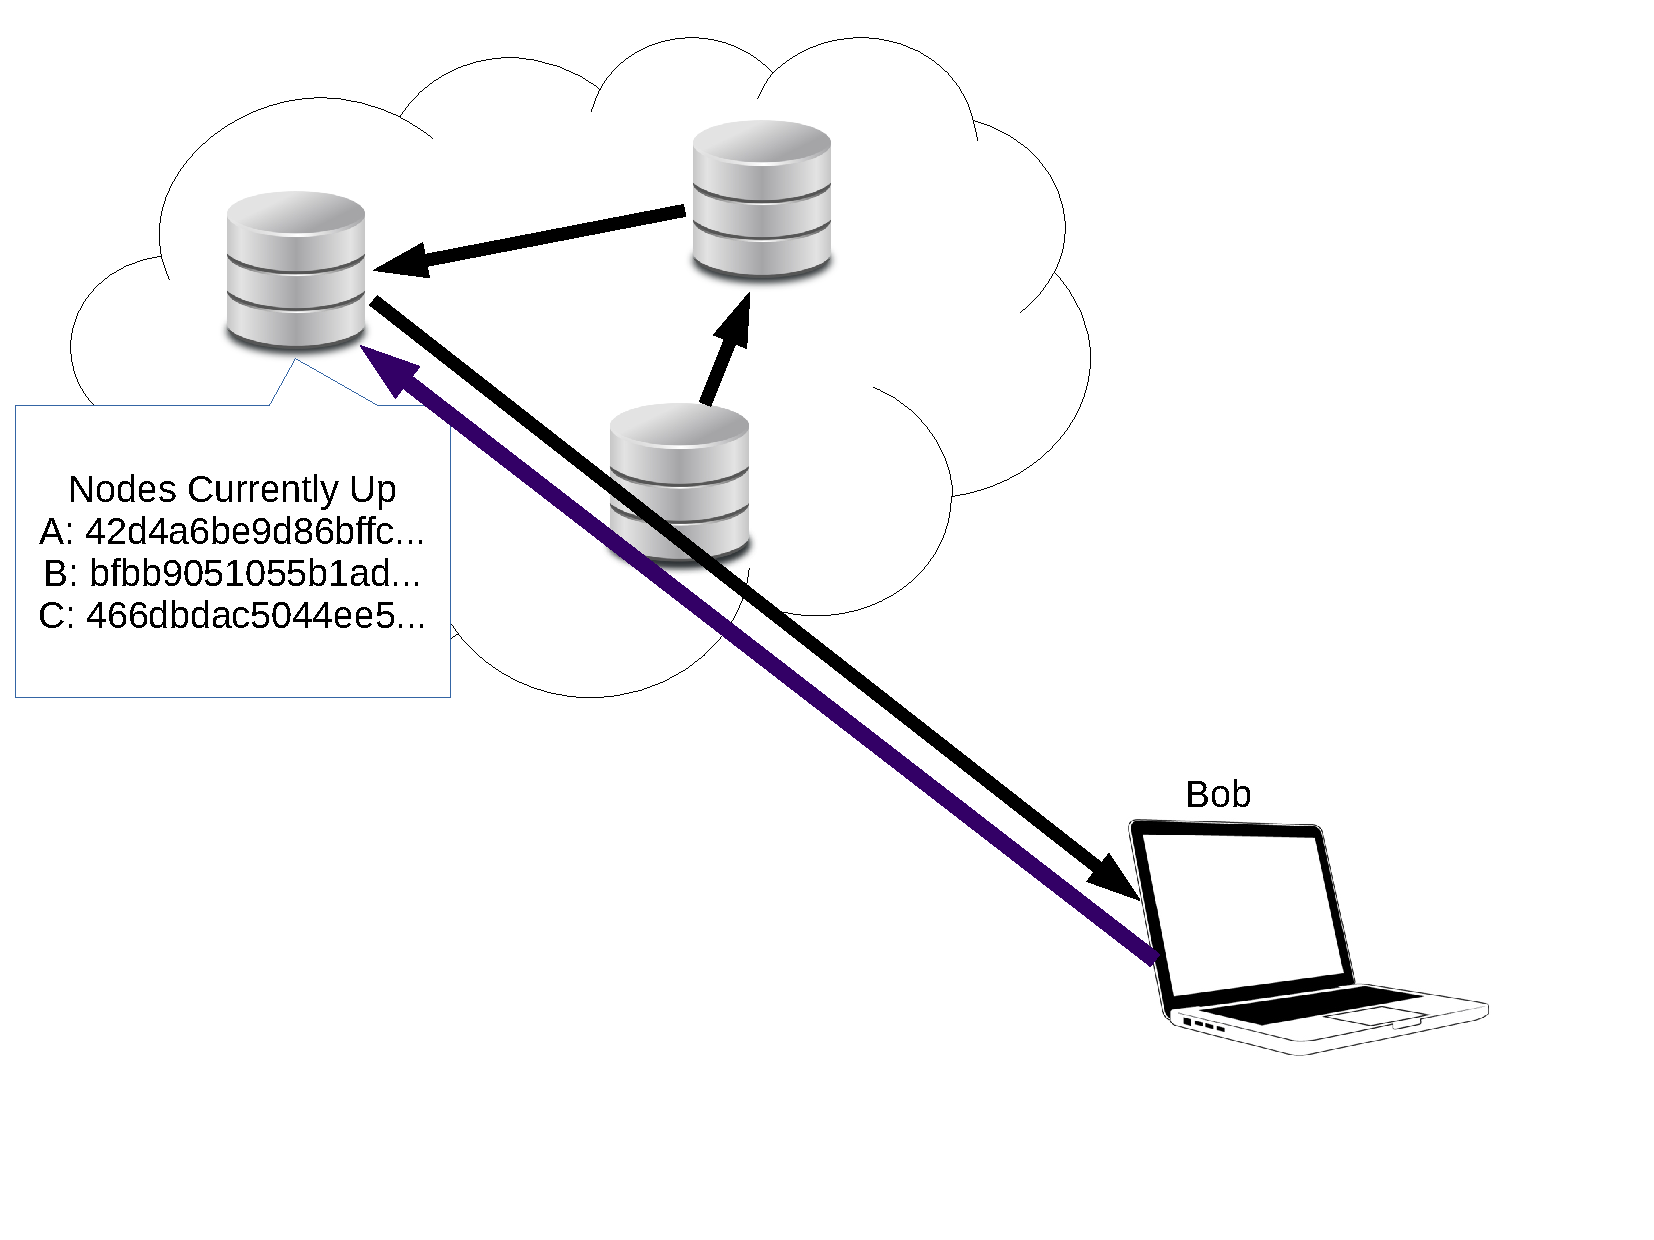
\includegraphics[scale=0.35]{figs/download.pdf}
    \\
    \small{Downloading from the service is equally user-friendly. A GET request is issued on the file's hash, and as multiple parts
    of the file trickle in, any missing pieces can be reconstructed via secret-sharing. As pieces either are pulled from the data store
    or reconstructed, a rolling checksum against the file's hash is performed, ensuring malicious add-ons are not incorporated into the
    reconstructed encrypted file. }
    \\
\end{center}

Bamboo underlies a nosqlesque key-value store application unrolled on each vps contribution

Updates to vps nodes are centrally controlled using github and implemented by users doing `git clone' and 'make'

We might also do something with puppet and/or rsync if needed but likely not

Everything is implemented on planetlab for now but more nodes will be added on actual vpses once we iron out those pesky details

Now for some stats and facts about our performance and possibly even our performance with routing algorithms other than Chord-FRT

Lastly we'll talk about what our next steps are


\section{Conclusions and Future Work}
\label{sec:concl}


In this paper we ...

Blah blah blah...

\pagebreak

%\footnotesize
\nocite{*}
\bibliography{refs}
\bibliographystyle{abbrv}

\end{document}
